\documentclass{beamer}
\usepackage{tikz}
\title{Rustc's MIR -- LLVM Course}
\date{October 31, 2016}
\author{Avi Weinstock}
\usepackage{fancyvrb}
\begin{document}
\maketitle

\begin{frame}[fragile]
\frametitle{What is Rust?}
\begin{itemize}
\item
Programming language from Mozilla Research
\item
Initial prototype in 2009, first stable release in May 2015
\item
Feels like a mix of Haskell \& C++
\item
Uses LLVM for optimization and codegen
\end{itemize}
\end{frame}

\begin{frame}[fragile]
\frametitle{Overview of rustc}
% wget https://blog.rust-lang.org/images/2016-04-MIR/flow.svg
% convert flow.svg flow.png
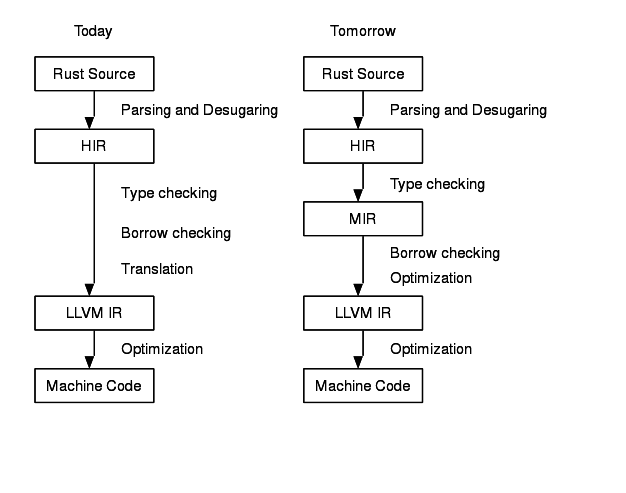
\includegraphics[width=0.9\textwidth]{flow.png}\\
\verb|https://blog.rust-lang.org/images/2016-04-MIR/flow.svg|
\end{frame}

\begin{frame}[fragile]
\frametitle{Code pointers}
\verb|https://github.com/rust-lang/rust|
\begin{itemize}
\item MIR definition: \verb|src/librustc/mir/mod.rs|
\item Borrowcheck: \verb|src/librustc_borrowck/borrowck/|\\\verb|{mod.rs,mir/mod.rs}|
\item Generation of LLVM IR: \verb|src/librustc_trans/|\\\verb|{base.rs,builder.rs,mir/mod.rs}|
\end{itemize}
\end{frame}

\begin{frame}[fragile]
\frametitle{Resources}
\begin{itemize}
\item \verb|https://blog.rust-lang.org/2016/04/19/MIR.html|
\item \verb|https://github.com/rust-lang/rfcs/|\\\verb|blob/master/text/1211-mir.md|
\item \verb|https://doc.rust-lang.org/book/|\\\verb|references-and-borrowing.html|
\item \verb|http://smallcultfollowing.com/babysteps/blog/|\\\verb|2016/04/27/non-lexical-lifetimes-introduction/|
\end{itemize}
\end{frame}

\end{document}
